%-----------------------------------------------------------------------------------
%	PACKAGES AND OTHER DOCUMENT CONFIGURATIONS
%----------------------------------------------------------------------------------

\documentclass[t,aspectratio=169]{beamer}

\usepackage{pgfpages}
%% \setbeameroption{show notes on second screen} % comment to hide 
\setbeamertemplate{note page}{\insertnote}


\newcommand{\Var}{\mathrm{Var}}

\newcommand{\Cov}{\mathrm{Cov}}

\newcommand{\plim}{\rightarrow_{p}}
\newcommand{\indep}{\perp \!\!\! \perp}

\usepackage[natbibapa]{apacite}
\usepackage{amsmath, amsfonts}
\usepackage{graphicx}
\usepackage{pdfpages}
\usepackage{bm}
\usepackage{listings}
\usepackage{multirow,array}
\usepackage{enumerate}
\usepackage{bbm}
%\usepackage{subfig}
\usepackage{bbm}
\usepackage{multirow}
\usepackage[space]{grffile}
\usepackage{subcaption}
\usepackage[utf8]{inputenc}
\usepackage{csquotes}
\usepackage{hyperref} 

\usepackage{amssymb}

\usepackage{mathrsfs}
\usepackage{float}
\usepackage{booktabs}
\usepackage{color}
\usepackage{rotating}
\usepackage{amsthm}
\usepackage{multirow,array}
\usepackage{caption}
\usepackage{url}
\usepackage[export]{adjustbox}
  \usepackage{multimedia}


\DeclareMathOperator*{\argmax}{arg\,max}
\DeclareMathOperator*{\argmin}{arg\,min}




% Expectation symbol
\newcommand{\E}{\mathrm{E}}
\newcommand{\V}{\mathrm{V}}
\newcommand{\N}{\mathcal{N}}
\newcommand{\R}{\mathbb{R}} 

\setbeamertemplate{navigation symbols}{}
\setbeamertemplate{footline}[frame number]

\setbeamertemplate{itemize items}[square]

\newtheorem{axiom}{Axiom}
\newtheorem{assump}{Assumption}

\setbeamertemplate{theorems}[numbered]

\setbeamerfont{title}{size=\huge}
\setbeamerfont{frametitle}{size=\huge}
\setbeamerfont{framesubtitle}{size=\large}

%  color theme 
%----------------------------
\definecolor{midnightblue}{rgb}{0.1, 0.1, 0.44}


\definecolor{ptlightblue}{RGB}{119,170,221}	  
\setbeamercolor{structure}{fg=midnightblue}




%-----------------------------
% title stuff 
%-------------------------


\title{From Value Added to Welfare Added: \\ A Social Planner Approach to Education Policy and Statistics}

\author{Tanner S Eastmond\thanks{Department of Economics, University of California, San Diego: \texttt{teastmond@ucsd.edu}, \texttt{jbetts@ucsd.edu}} \and Nathan Mather\thanks{Department of Economics University of Michigan: \texttt{njmather@umich.edu}, \texttt{ricksmi@umich.edu}} \and Michael David Ricks$^2$ \and Julian Betts$^1$}


%----------------%
% Notes to self %
%-------------------%


%------------------------------------------------------------------------------
%	begin doc
%------------------------------------------------------------------------------

\begin{document}



%------------------------------------------------------------------------
% Intro 
%------------------------------------------------------------------------
    
 \frame{\titlepage}

 %--------------------------------------------------------
 % General idea 
 \begin{frame}{Introduction}

    \begin{itemize}
        \vspace{.75em}
        \setlength\itemsep{.75em}
        \item Average's might not be sufficient for recovering welfare from any policy 
        \item Value added uses average test score gains 
        \item We look at test score gains across achievement distribution 
        \item Theory connects welfare impact of education policy to test scores
        \begin{itemize}
            \vspace{.4em}
            \setlength\itemsep{.4em}
            \item When does heterogeneity of teacher ability matter for predicting average policy impact 
            \item When does measuring heterogeneity of policy impact matter 
        \end{itemize}
        \item Show heterogeneity exists 
        \item Show we can measure it
        \item Show Production Possibility frontier for teacher reassignment 
        \item Show how standard value added misranks teachers
    \end{itemize}
     
 \end{frame}

%------------------------------------------------------------
% MOdel 
%------------------------------------------------------------

      %------------------------------------------------------------
    % Model: Deconstructing Value Added 
    \begin{frame}{Value Added Deconstruction}

    let $A_j = \omega_{0}\alpha_{j,0} + \omega_{1}\alpha_{j,1}$ 
    
    let $C_j = \alpha_{j,1} - \alpha_{j,0}$

    \vspace{1em}
    \textbf{Deconstructing value added gives:}
            \begin{align*}
            \alpha_j  &= \omega_{j,0}(\mu_0 +\alpha_{j,0}) + \omega_{j,1}(\mu_1 +\alpha_{j,1})  \\
                      &  =  A_j  + C_j  ( \omega_{j,1} - \omega_{j,0} ) + \sum_k  \omega_{j,k} \mu_k
        \end{align*}

    
        This has three components: the absolute average impact, the allocative efficiency (comparative advantage times the relative matched proportion), and the classroom average of population residuals.
        
    \end{frame}
     
    %------------------------------------------------------------
    % Model: Utility and Test Scores 
    \begin{frame}{Model: Utility and Test Scores}
    \vspace{2em}
    \textbf{Policymaker's Goal}
    \begin{equation}
        \max \sum_i \E[ \psi_i U_{i} |S_{it}]
    \end{equation}
    
    \vspace{3em
    }
    \textbf{Put in terms of policy's impact on test scores }
        \begin{equation}
            \E[\psi_i U_i|S_{it}] - \E[\psi_i U_i |S_{i,t-1}] =  \frac{\E[\psi_i U_i|S_{it}] - \E[\psi_i U_i |S_{i,t-1}] }{\Delta^jS_i} \Delta^jS_i = \gamma_i(S_{it}, S_{i,t-1}) \Delta^jS_i
        \end{equation}
     
    \end{frame}
        


    %------------------------------------------------------------
    % Model: Policy Heterogeneity 
    \begin{frame}{Welfare of a Policy Change }

let $\gamma_i = \gamma$ i.e. welfare weights are only a function of test scores. Then condition on observables S_{i,t-1}, X_i

\vspace{1em}
    \textbf{Definition 3:}
                If $ \gamma(S_{it}, S_{i,t-1}) \indep \Delta S_i^j |S_{i,t-1}, X_i $ then
            \begin{equation*}
               \E[\sum_i \gamma(S_{it}, S_{i,t-1})) \Delta S_i^j| S_{i,t-1}, X_i]= \sum_i \: \E[\gamma(S_{it}, S_{i,t-1}))|S_{i,t-1}, X_i] \:\E[\Delta S_i^j|S_{i,t-1}, X_i] 
            \end{equation*}

            \vspace{1em}

    \textbf{Connected to VAM}
    \begin{align*}
      \\ = \sum_i \: \E[\gamma(S_{i,t-1} + \hat{\alpha}_{j,i}, S_{i,t-1})] \hat{\alpha}_{j,i}
    \end{align*}

    \end{frame}


 %------------------------------------------------------------
% Data 
%------------------------------------------------------------

\begin{frame}{Data}
\begin{itemize}
        \vspace{.75em}
        \setlength\itemsep{.75em}
    \item Administrative data on universe students in San Diego Unified School District

    \item Main Sample: 2,165 teachers teaching grades 3-5
        
    \begin{itemize}
            \vspace{.5em}
        \setlength\itemsep{.5em}
        \item Restrict to school years between spring 2003 and 2013 (long term effects)
        \item Require that students have test scores for consecutive years (to estimate VA)
        \item Require that a teacher teaches at least 50 such students (to power heterogeneity)
    \end{itemize}    
        
    \item SDUSD has rich data on many variables of interests
        \begin{itemize}
                \vspace{.5em}
        \setlength\itemsep{.5em}
        \item Math and ELA scores, standardized to the mean and variance of California
        \item Long term outcomes: graduation, college enrollment, degree completion
        \item Controls for student characteristics and lagged student, class, and school achievement
    \end{itemize}  
\end{itemize}
\end{frame}

 %------------------------------------------------------------
% Emperical Results 
%------------------------------------------------------------

\begin{frame}{Results: long term outcomes}
    \begin{center}
    \resizebox{!}{.02\textwidth}{
    $y_{i,j} = \sum_{k_j,k_i} \tau_{k_j,k_i} \hat{\gamma}_{j,k_j}\mathds{1}(k(i) = k_i) + \beta_2 X_i + \nu_{i,j}$}
    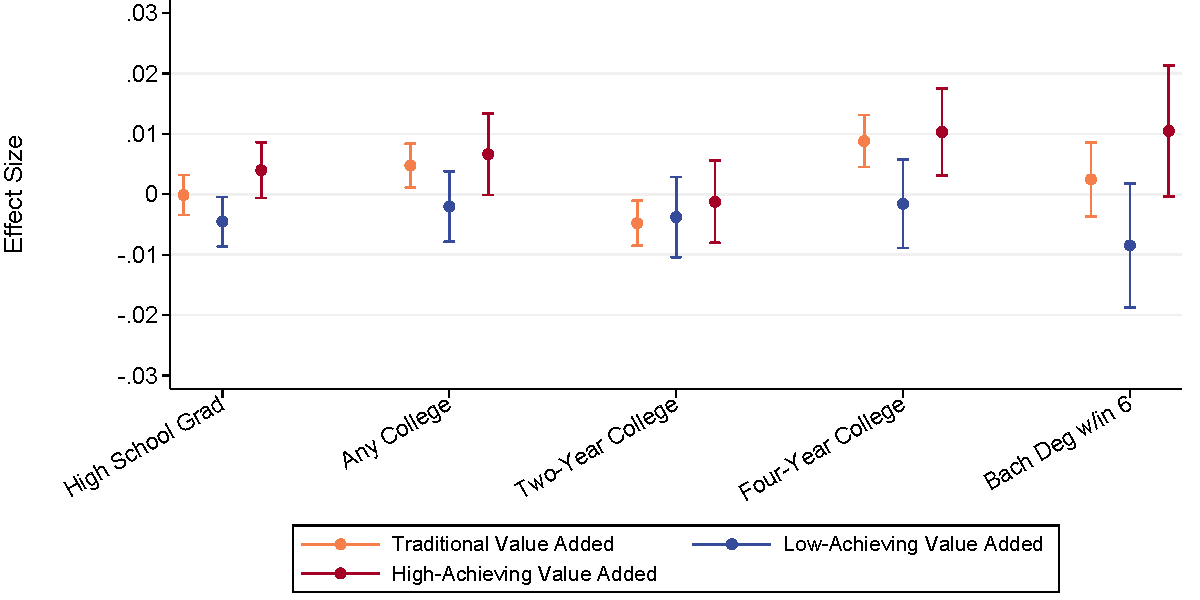
\includegraphics[width=.9\textwidth]{Working_Paper/WP_Figures/fig2b_longterm.pdf}
    \end{center}

\end{frame}


\begin{frame}{Results: PPFs}
\begin{figure}[H]
    \centering
    \resizebox{.3\textwidth}{!}{$\max_\mathcal{J} \mathcal{W}(\mathcal{J}) =  \sum_j \sum_{i\in j} \omega_{k(i)} \alpha_{j,{k(i)}}$}
    
    \begin{subfigure}[b]{0.45\textwidth}
    \subcaption[]{Within School ELA}
        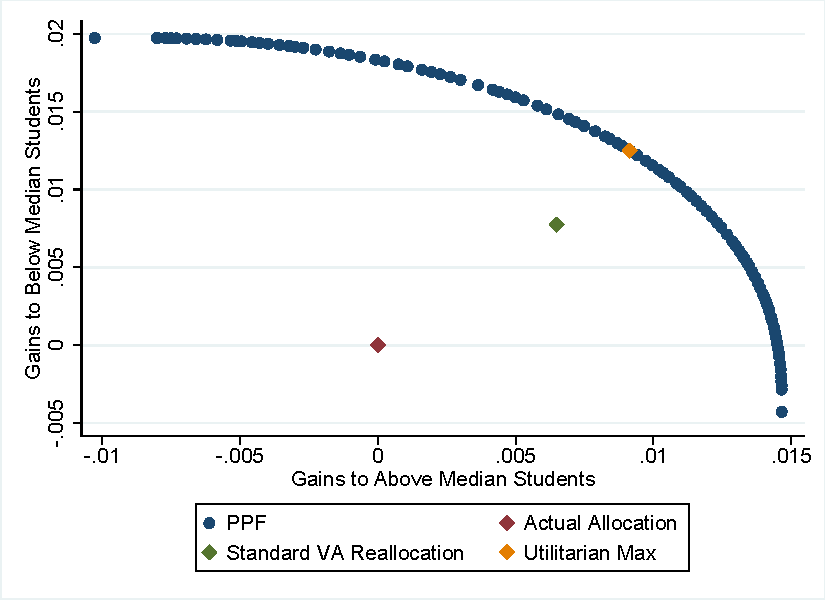
\includegraphics[width=1\textwidth]{Working_Paper/WP_Figures/WithinSchoolReallocationELA.pdf}
    \end{subfigure}
    \begin{subfigure}[b]{0.45\textwidth}
    \subcaption[]{Within School Math}
        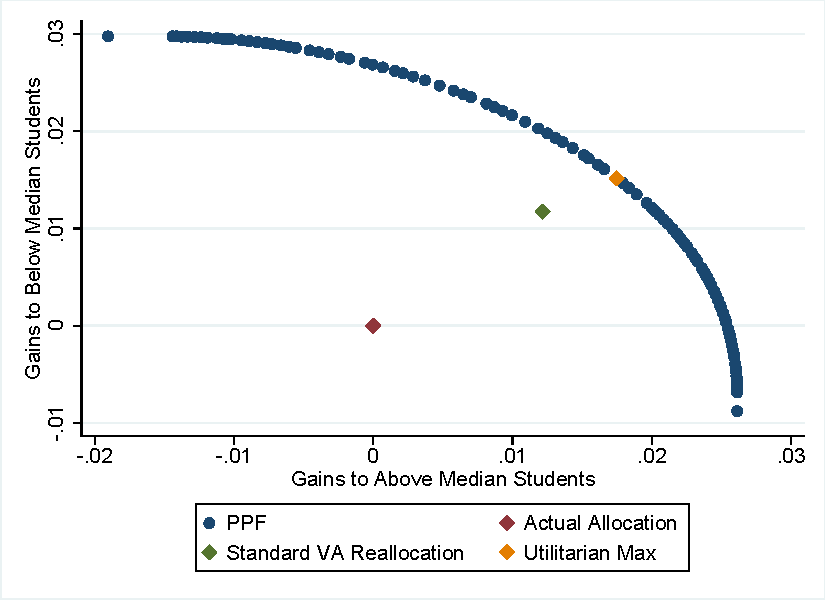
\includegraphics[width=1\textwidth]{Working_Paper/WP_Figures/WithinSchoolReallocationMath.pdf}
    \end{subfigure}
\end{figure}

\end{frame}


\begin{frame}{Results: PPFs}
\begin{figure}[H]
    \centering
    \resizebox{.3\textwidth}{!}{$\max_\mathcal{J} \mathcal{W}(\mathcal{J}) =  \sum_j \sum_{i\in j} \omega_{k(i)} \alpha_{j,{k(i)}}$}
    
    \begin{subfigure}[b]{0.45\textwidth}
    \subcaption[]{Across School ELA}
        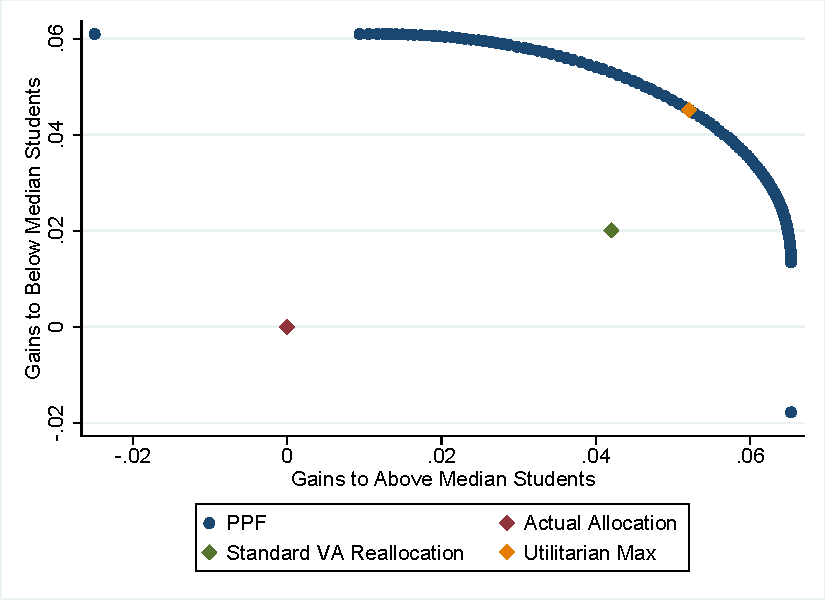
\includegraphics[width=1\textwidth]{Working_Paper/WP_Figures/AcrossSchoolReallocationELA.pdf}
    \end{subfigure}
    \begin{subfigure}[b]{0.45\textwidth}
    \subcaption[]{Across School Math}
        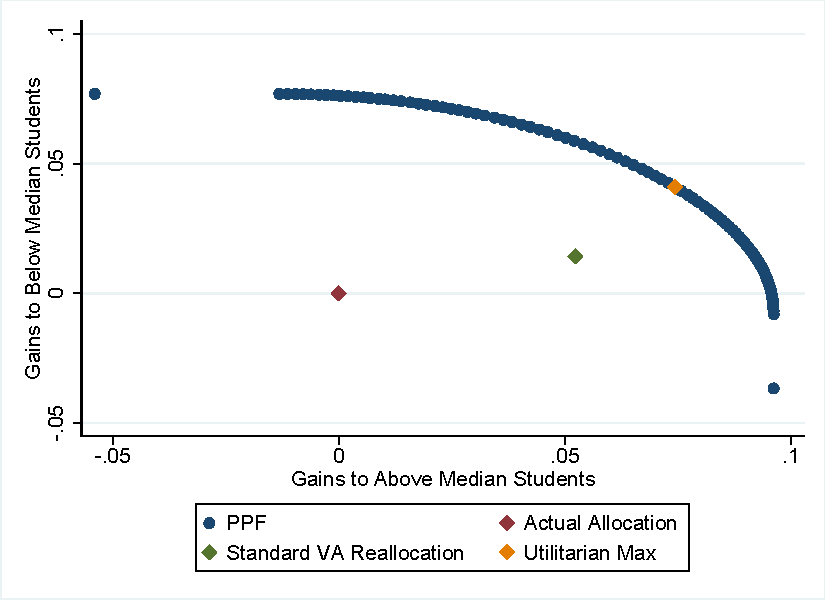
\includegraphics[width=1\textwidth]{Working_Paper/WP_Figures/AcrossSchoolReallocationMath.pdf}
    \end{subfigure}
\end{figure}

\end{frame}


\begin{frame}{Results: Disparities}

    \begin{figure}[H]
        \centering
          \centering
         \begin{subfigure}[b]{0.45\textwidth}
        \subcaption[]{High and Low Test Score Gaps}
            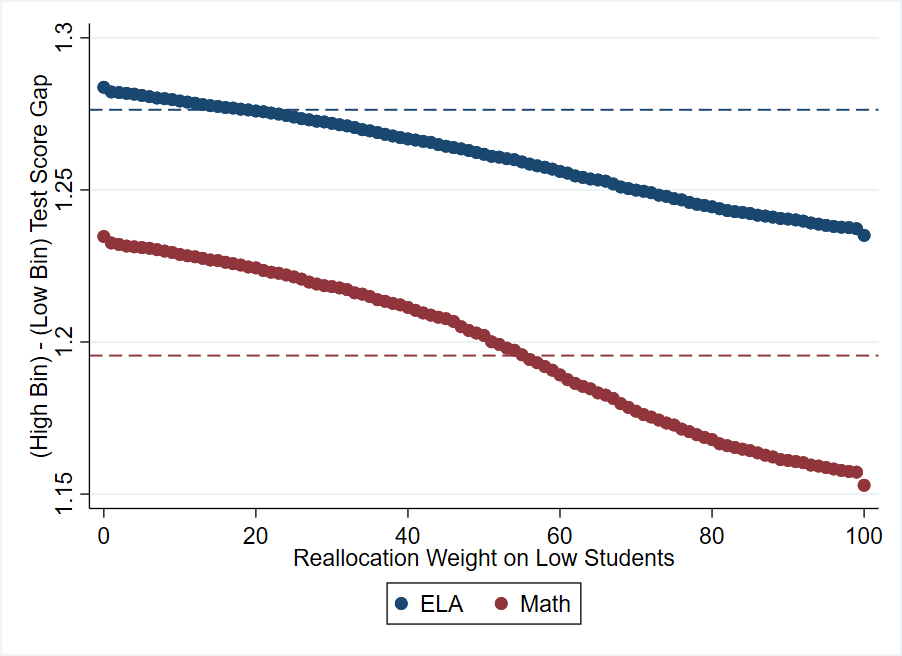
\includegraphics[width=1\textwidth]{Working_Paper/WP_Figures/test_score_gaps.png}
        \end{subfigure}
        \begin{subfigure}[b]{0.45\textwidth}
        \subcaption[]{Racial Gaps}
            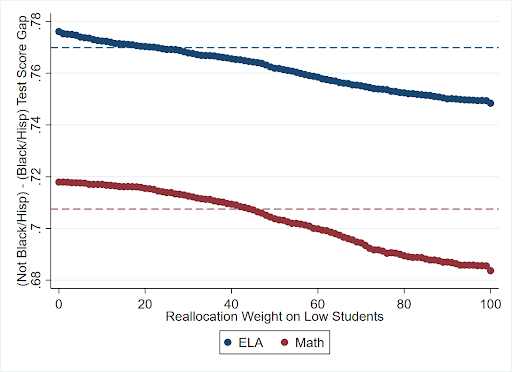
\includegraphics[width=1\textwidth]{Working_Paper/WP_Figures/race_gaps.png}
        \end{subfigure}
    \end{figure}
    
\end{frame}
 %------------------------------------------------------------
% conclusion 
%------------------------------------------------------------

  
\begin{frame}{Conclusion}

    \begin{itemize}
        \vspace{1em}
        \setlength\itemsep{1em}
        \item Average effects often aren't enough for decision makers to recover welfare 
        \item Measuring heterogeneity can give more accurate estimates of mean impact
        \item If welfare weights differ, conditional policy impact is important
        \item Measuring heterogeneity in value added is possible 
        \item Measuring heterogeneity better shows the range of possible policy outcomes

    \end{itemize}
\end{frame}
  
  
%------------------------------------------------------------------------
% citations
%------------------------------------------------------------------------

\begin{frame}{Citations}
\bibliographystyle{apacite}
\bibliography{References}
\end{frame}

  
%------------------------------------------------------------------------
% appendix slides 
%------------------------------------------------------------------------

\begin{frame}[noframenumbering]{Appendix}
\label{}

\end{frame}

%------------------------------------------------
% end doc
%------------------------------------------------
\end{document}

